\chapter{Informations}

\section{La page "Statistiques"}
Sur cette page sont présentées des statistiques sur les ventes.

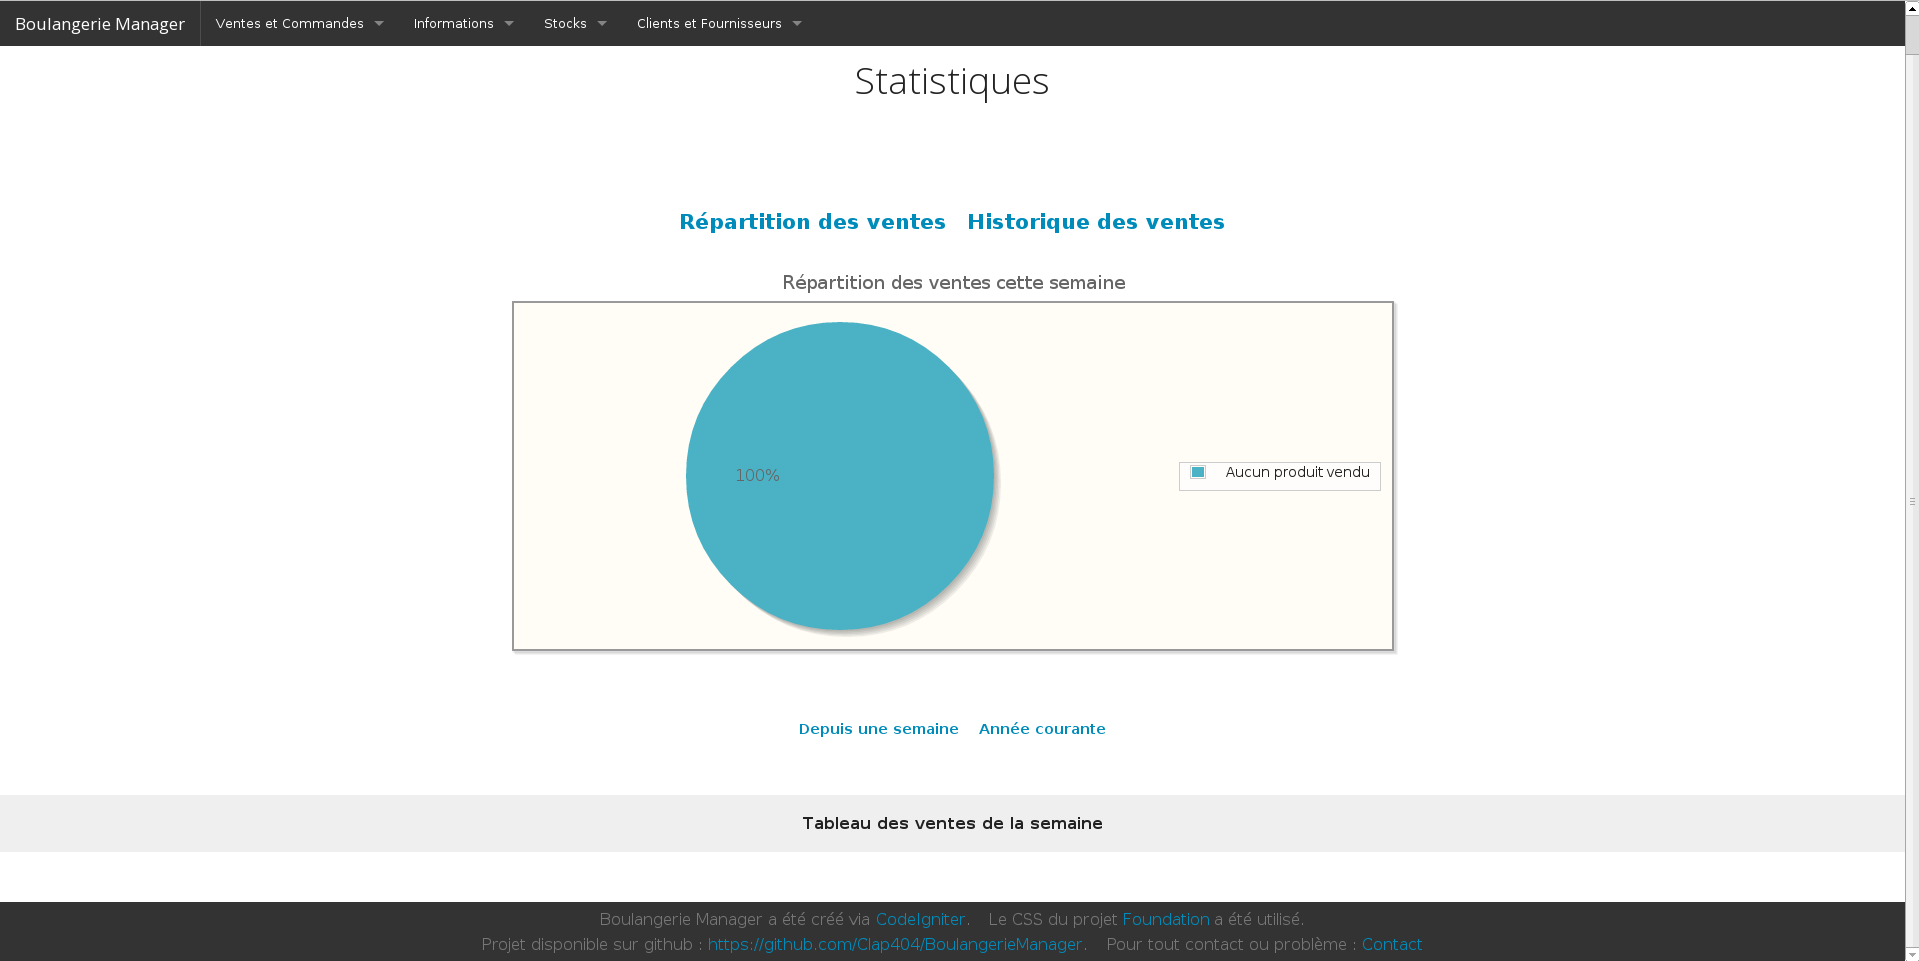
\includegraphics[scale=0.30]{stats1.png}
\paragraph{}
Sur la page "Statistiques" se trouve un diagramme circulaire présentant la
répartition des ventes de cette semaine en fonction du type de produit. Sous
ce graphique on peut trouver un bouton "Depuis une semaine" et un autre bouton
"Année Courante". Ces deux boutons permettent de naviguer entre le diagramme
représentant les ventes de la semaine en cours ainsi que celui représentant la
répartition des ventes de l'année courante.\\

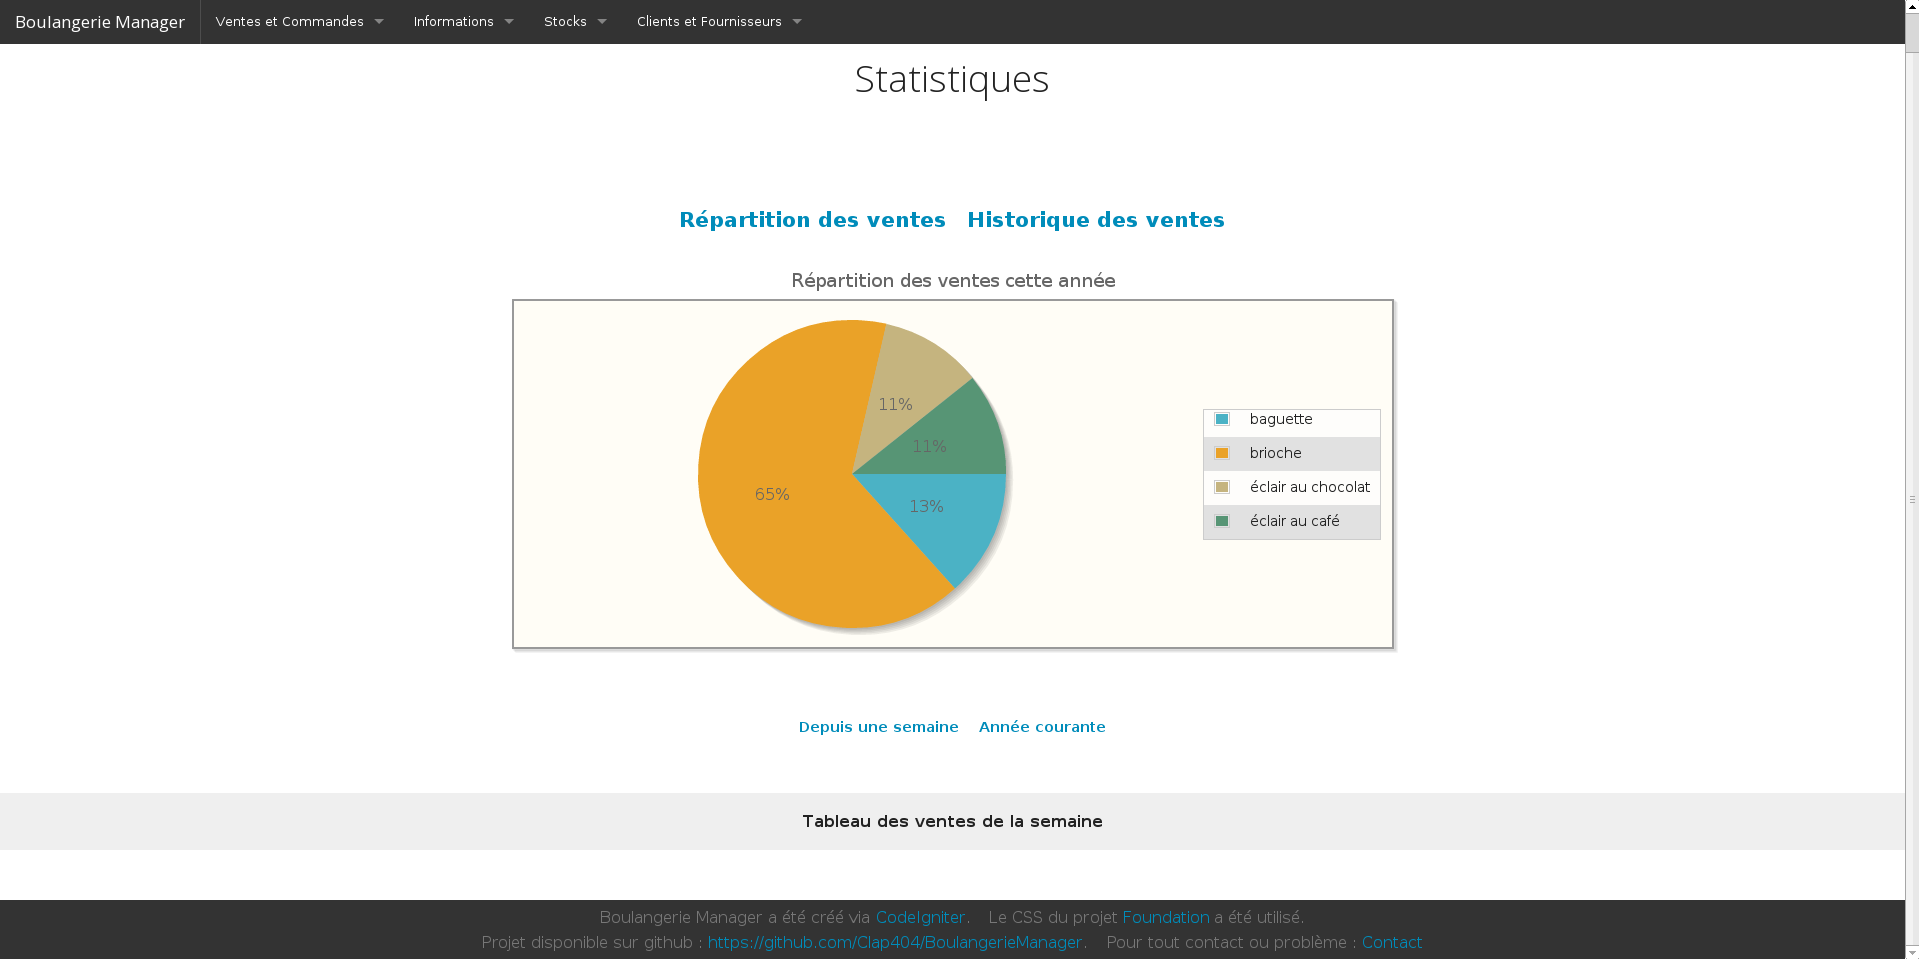
\includegraphics[scale=0.30]{stats3.png}

\paragraph{}
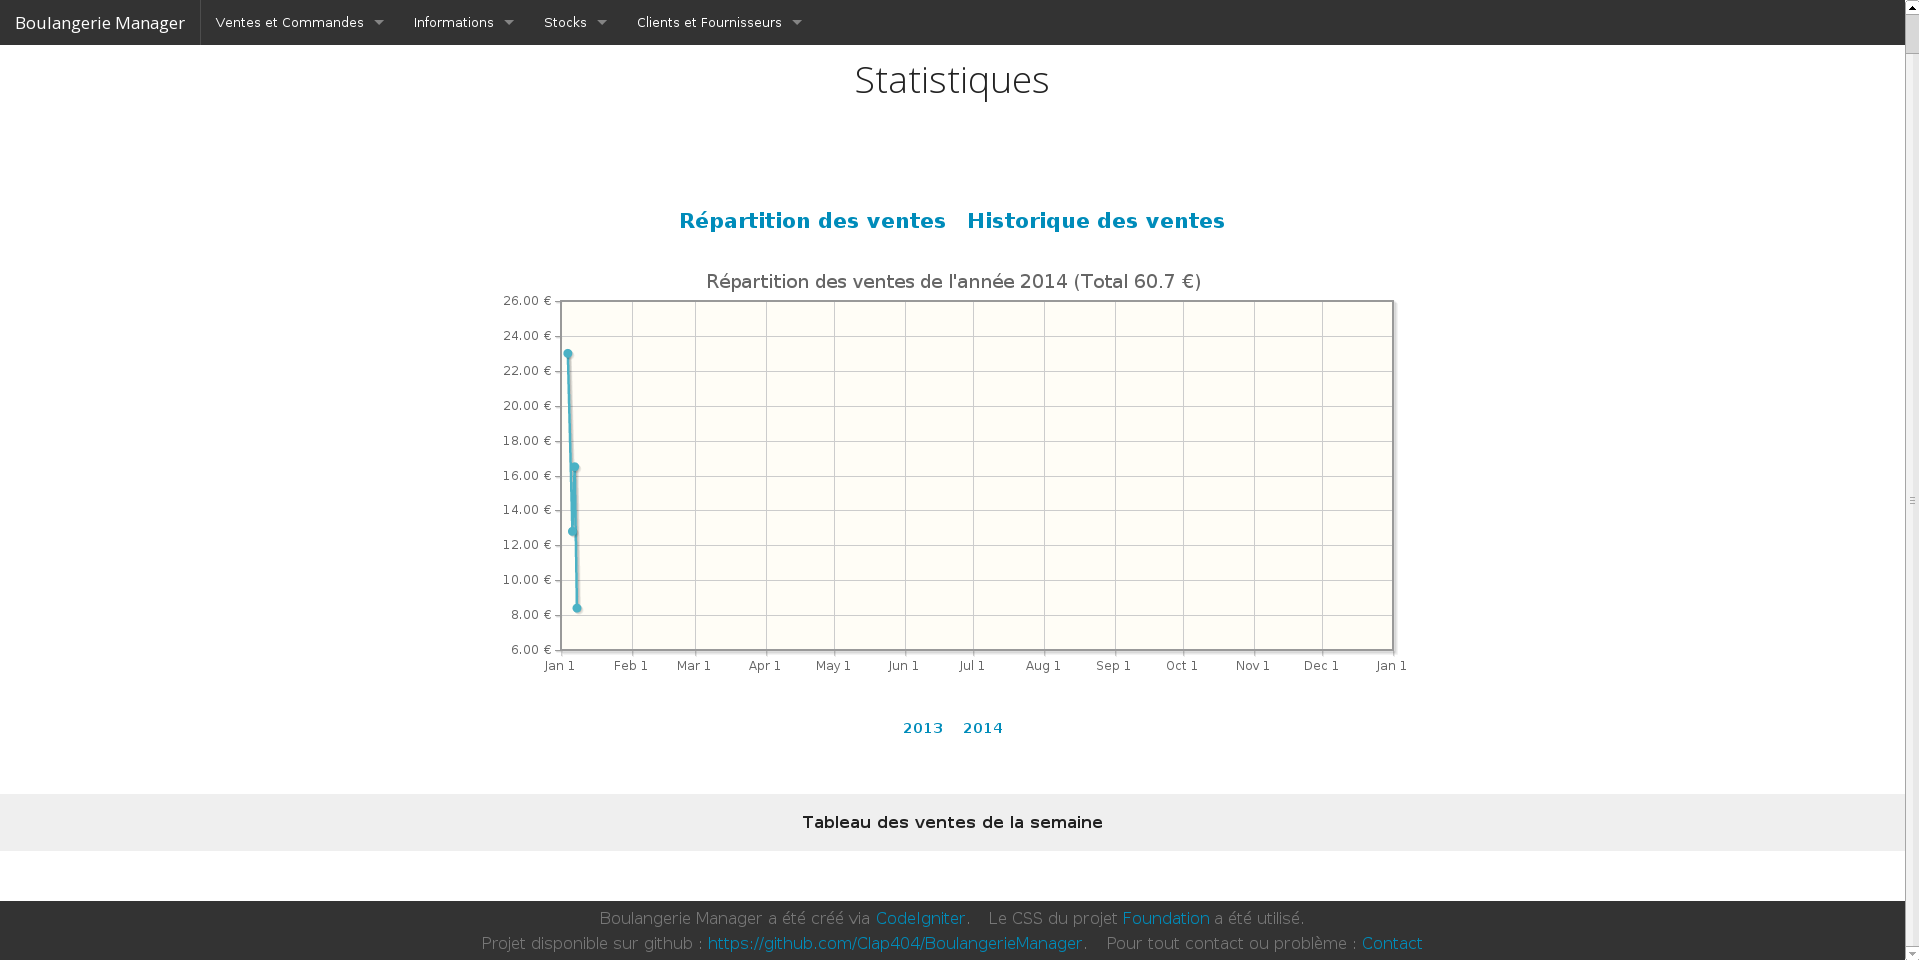
\includegraphics[scale=0.30]{stats2.png}\\
Sur cette même page se trouve un bouton "Historique des ventes". Un clic sur ce
bouton permet d'afficher un historique des ventes en fonction des années,
grâce à une courbe. Sous cette courbe se situent alors des boutons représentant
les différentes années pendant lesquelles on peut observer l'évolution des ventes.

\paragraph{}
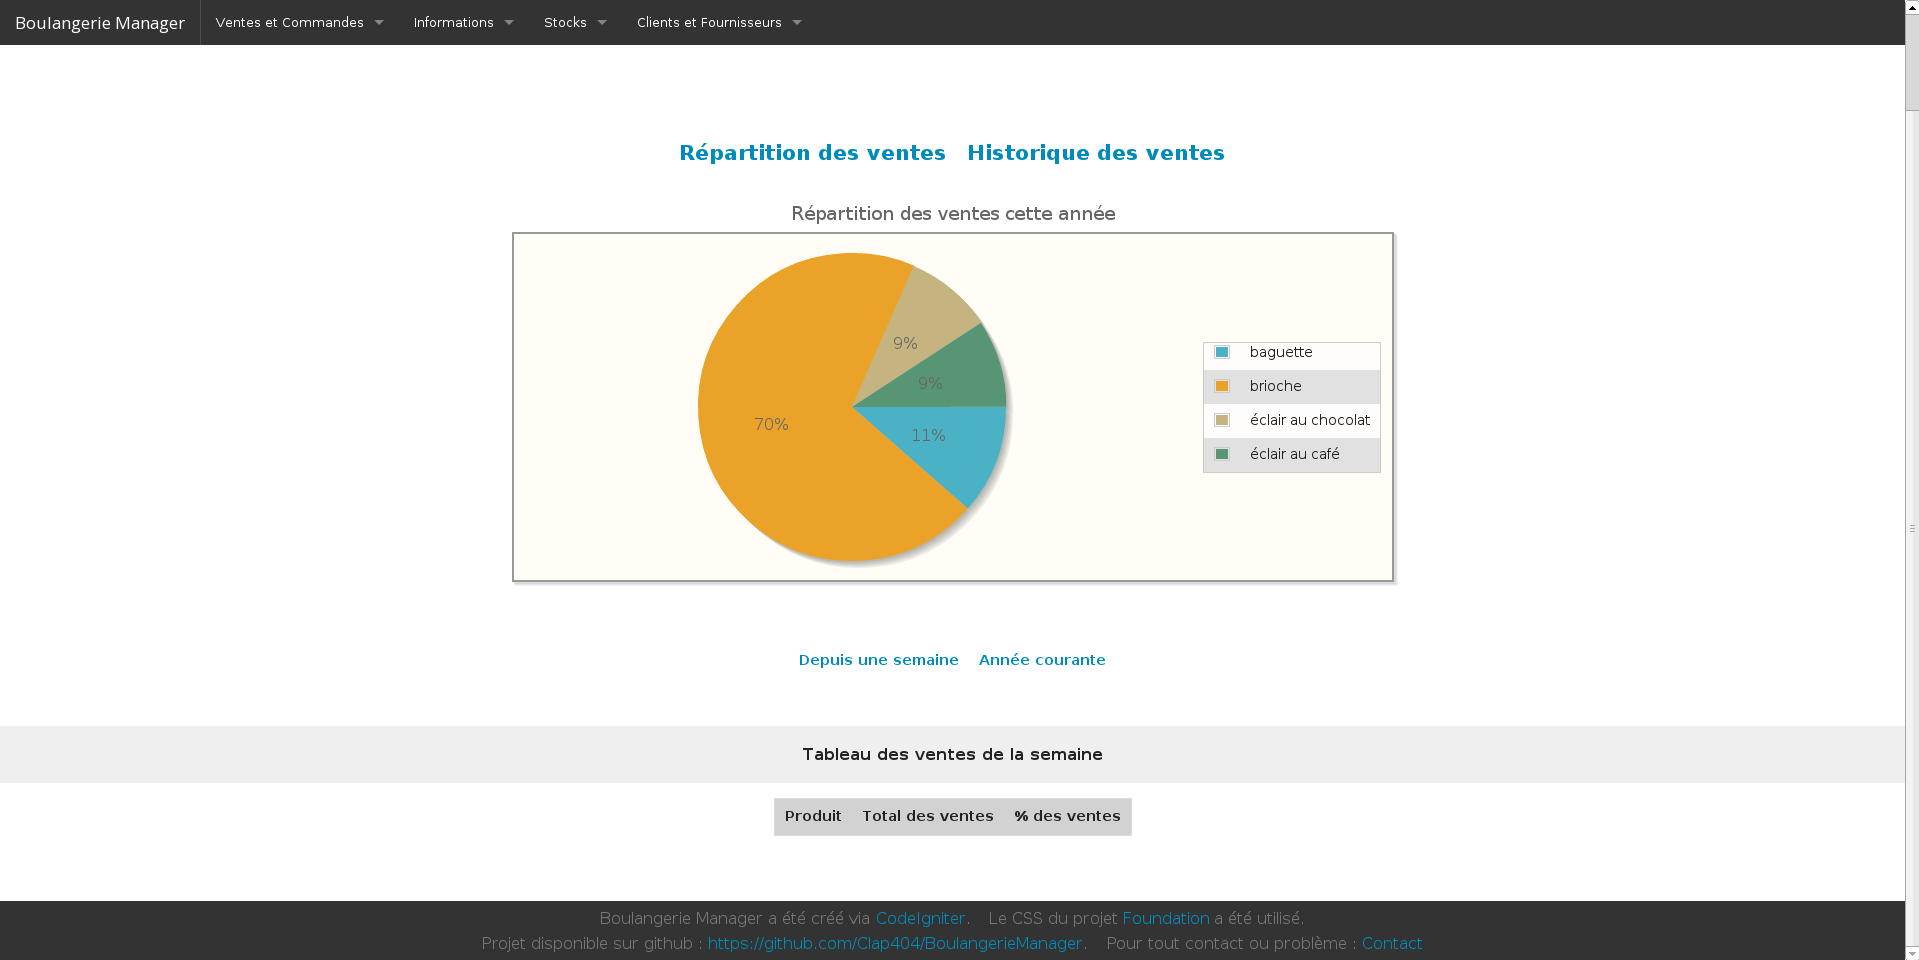
\includegraphics[scale=0.30]{stats4.png}\\
En dessous de ce graphique, une barre déroulante "Tableau des ventes de la
semaine" est présente. En cliquant sur cette barre, un tableau apparaît
représentant les ventes de la semaine. Ce tableau contient les noms des
produits, le total des ventes depuis le début de la semaine ainsi que le
pourcentage que cela représente par rapport au total des ventes, sur la même
période. Un autre clic sur cette barre masque le tableau à nouveau.



\section{La page "Invendus"}
Dans cette page sont présentés tous les invendus.\\
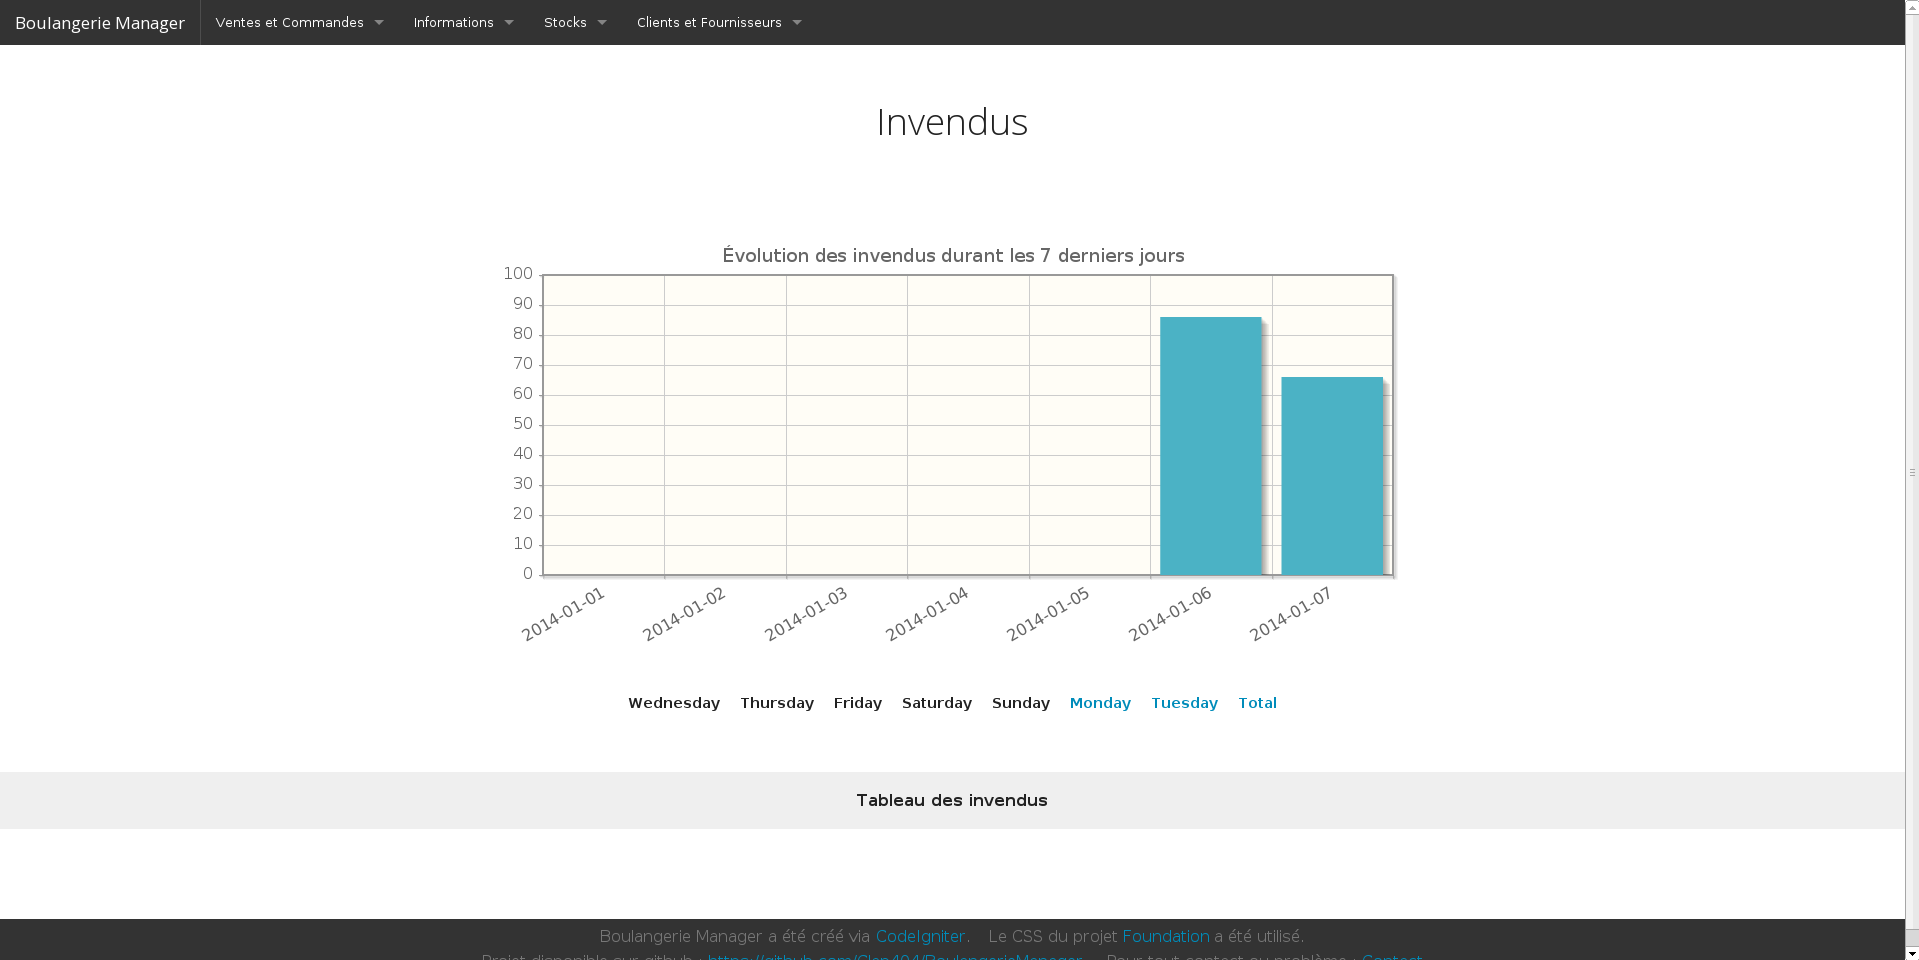
\includegraphics[scale=0.30]{invendus1.png}
\paragraph{}
Sur la page "Invendus" se trouve un graphique présentant l'évolution des produits
invendus durant les sept derniers jours. Il est possible de cliquer sur les
jours pendant lesquels des produits sont restés invendus.\\
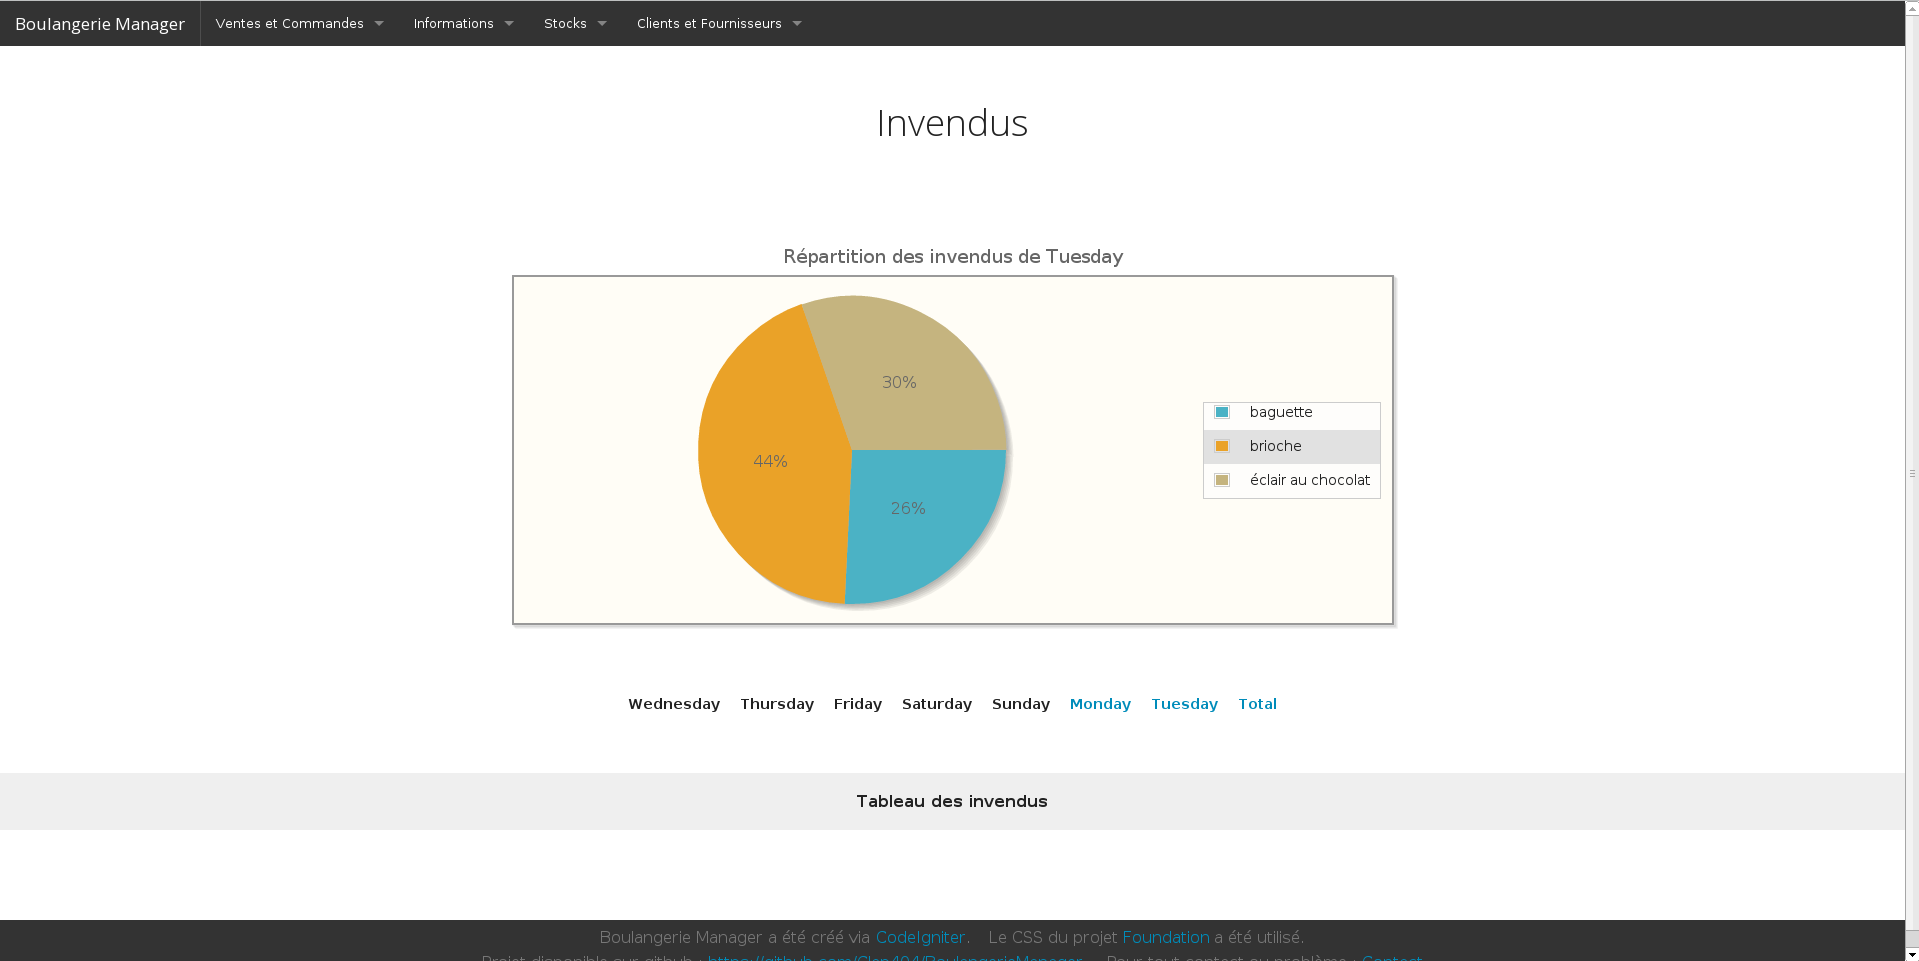
\includegraphics[scale=0.30]{invendus2.png}
\paragraph{}
En cliquant sur un jour, un diagramme circulaire s'affiche représentant la part de chaque produit dans les
invendus du jour. Dans ce graphique se trouve une légende qui liste les
différentes couleurs associées aux produits invendus. Un clic sur le bouton
"Total" permet à tout moment de revenir au graphique représentant l'évolution
sur les sept derniers jours.\\
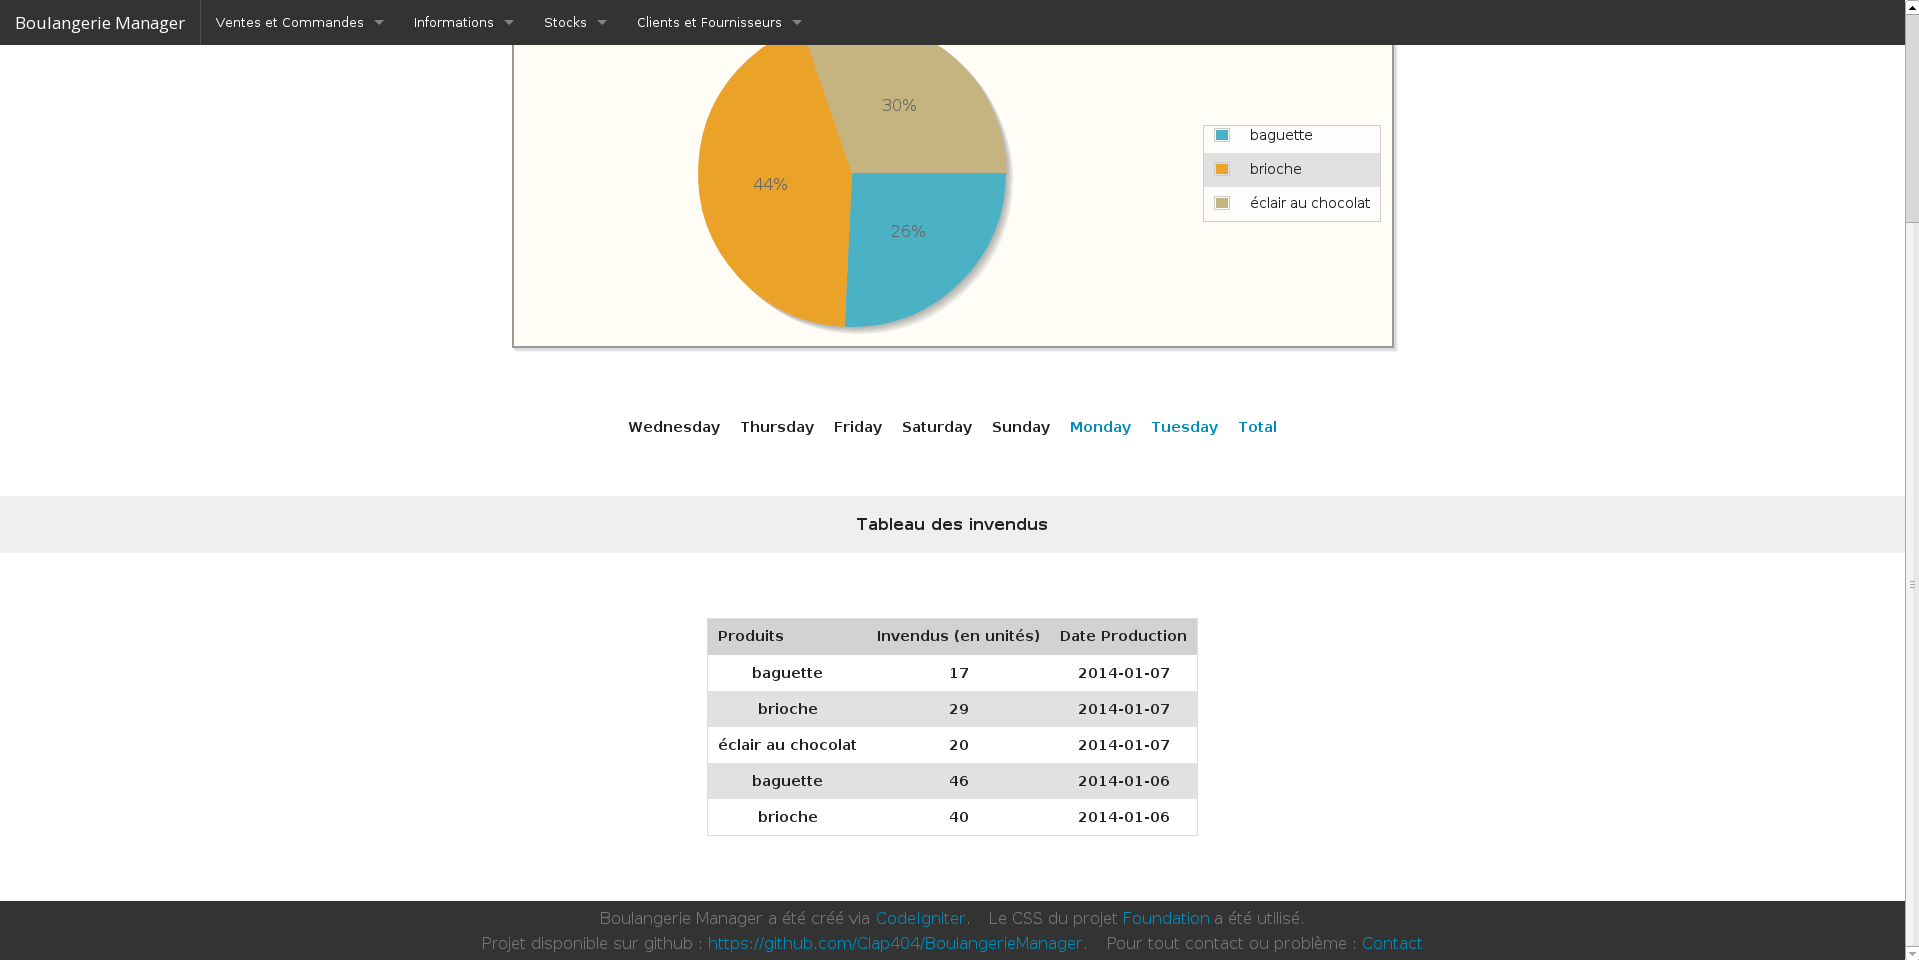
\includegraphics[scale=0.30]{invendus3.png}
\paragraph{}
En dessous de ce graphique, une barre déroulante "Tableau des invendus" est
présente. En cliquant sur cette barre, un tableau apparaît représentant les
invendus sur les sept derniers jours. Dans ce tableau sont renseignés les noms
des produits, la quantité d'invendus ainsi que la date de production de ceux-ci.
Un second clic sur la barre déroulante masque le tableau à nouveau.
